\documentclass[journal,12pt,twocolumn]{IEEEtran}

\usepackage{setspace}
\usepackage{gensymb}

\singlespacing


\usepackage[cmex10]{amsmath}

\usepackage{amsthm}
\usepackage{amsmath}
\usepackage{mathrsfs}
\usepackage{txfonts}
\usepackage{stfloats}
\usepackage{bm}
\usepackage{cite}
\usepackage{cases}
\usepackage{subfig}


\usepackage{longtable}
\usepackage{multirow}

\usepackage{enumitem}
\usepackage{mathtools}
\usepackage{steinmetz}
\usepackage{tikz}
\usepackage{circuitikz}
\usepackage{verbatim}
\usepackage{tfrupee}
\usepackage[breaklinks=true]{hyperref}
\raggedbottom

\usepackage{tkz-euclide}
\usepackage{caption}
\usepackage{wrapfig}

\usetikzlibrary{calc,math}
\usepackage{listings}
    \usepackage{color}                                            %%
    \usepackage{array}                                            %%
    \usepackage{longtable}                                        %%
    \usepackage{calc}                                             %%
    \usepackage{multirow}                                         %%
    \usepackage{hhline}                                           %%
    \usepackage{ifthen}                                           %%
    \usepackage{lscape}     
\usepackage{multicol}
\usepackage{chngcntr}
\graphicspath{ {./images/} }

\DeclareMathOperator*{\Res}{Res}

\renewcommand\thesection{\arabic{section}}
\renewcommand\thesubsection{\thesection.\arabic{subsection}}
\renewcommand\thesubsubsection{\thesubsection.\arabic{subsubsection}}

\renewcommand\thesectiondis{\arabic{section}}
\renewcommand\thesubsectiondis{\thesectiondis.\arabic{subsection}}
\renewcommand\thesubsubsectiondis{\thesubsectiondis.\arabic{subsubsection}}


\hyphenation{op-tical net-works semi-conduc-tor}
\def\inputGnumericTable{}                                 %%

\lstset{
%language=C,
frame=single, 
breaklines=true,
columns=fullflexible
}
\begin{document}


\newtheorem{theorem}{Theorem}[section]
\newtheorem{problem}{Problem}
\newtheorem{proposition}{Proposition}[section]
\newtheorem{lemma}{Lemma}[section]
\newtheorem{corollary}[theorem]{Corollary}
\newtheorem{example}{Example}[section]
\newtheorem{definition}[problem]{Definition}

\newcommand{\BEQA}{\begin{eqnarray}}
\newcommand{\EEQA}{\end{eqnarray}}
\newcommand{\define}{\stackrel{\triangle}{=}}
\bibliographystyle{IEEEtran}
\providecommand{\mbf}{\mathbf}
\providecommand{\pr}[1]{\ensuremath{\Pr\left(#1\right)}}
\providecommand{\qfunc}[1]{\ensuremath{Q\left(#1\right)}}
\providecommand{\sbrak}[1]{\ensuremath{{}\left[#1\right]}}
\providecommand{\lsbrak}[1]{\ensuremath{{}\left[#1\right.}}
\providecommand{\rsbrak}[1]{\ensuremath{{}\left.#1\right]}}
\providecommand{\brak}[1]{\ensuremath{\left(#1\right)}}
\providecommand{\lbrak}[1]{\ensuremath{\left(#1\right.}}
\providecommand{\rbrak}[1]{\ensuremath{\left.#1\right)}}
\providecommand{\cbrak}[1]{\ensuremath{\left\{#1\right\}}}
\providecommand{\lcbrak}[1]{\ensuremath{\left\{#1\right.}}
\providecommand{\rcbrak}[1]{\ensuremath{\left.#1\right\}}}
\theoremstyle{remark}
\newtheorem{rem}{Remark}
\newcommand{\sgn}{\mathop{\mathrm{sgn}}}
\providecommand{\abs}[1]{\left\vert#1\right\vert}
\providecommand{\res}[1]{\Res\displaylimits_{#1}} 
\providecommand{\norm}[1]{\left\lVert#1\right\rVert}
%\providecommand{\norm}[1]{\lVert#1\rVert}
\providecommand{\mtx}[1]{\mathbf{#1}}
\providecommand{\mean}[1]{E\left[ #1 \right]}
\providecommand{\fourier}{\overset{\mathcal{F}}{ \rightleftharpoons}}
%\providecommand{\hilbert}{\overset{\mathcal{H}}{ \rightleftharpoons}}
\providecommand{\system}{\overset{\mathcal{H}}{ \longleftrightarrow}}
    %\newcommand{\solution}[2]{\textbf{Solution:}{#1}}
\newcommand{\solution}{\noindent \textbf{Solution: }}
\newcommand{\cosec}{\,\text{cosec}\,}
\providecommand{\dec}[2]{\ensuremath{\overset{#1}{\underset{#2}{\gtrless}}}}
\newcommand{\myvec}[1]{\ensuremath{\begin{pmatrix}#1\end{pmatrix}}}
\newcommand{\mydet}[1]{\ensuremath{\begin{vmatrix}#1\end{vmatrix}}}
\numberwithin{equation}{subsection}
\makeatletter
\@addtoreset{figure}{problem}
\makeatother
\let\StandardTheFigure\thefigure
\let\vec\mathbf
\renewcommand{\thefigure}{\theproblem}
\def\putbox#1#2#3{\makebox[0in][l]{\makebox[#1][l]{}\raisebox{\baselineskip}[0in][0in]{\raisebox{#2}[0in][0in]{#3}}}}
     \def\rightbox#1{\makebox[0in][r]{#1}}
     \def\centbox#1{\makebox[0in]{#1}}
     \def\topbox#1{\raisebox{-\baselineskip}[0in][0in]{#1}}
     \def\midbox#1{\raisebox{-0.5\baselineskip}[0in][0in]{#1}}
\vspace{3cm}
\title{ASSIGNMENT 2}
\author{NSV SARATH CHANDRA(CC20MTECH14001)}
\maketitle
\newpage
\bigskip
\renewcommand{\thefigure}{\theenumi}
\renewcommand{\thetable}{\theenumi}
    
\section{Problem}
Using Baudhayana's theorem, show that \myvec{-3\\-4}, \myvec{2\\6} and \myvec{-6\\10} are the vertices of a right angled triangle. Repeat using orthogonality.  
% Check which of the following are solutions of the following equation:
% \begin{align} \myvec{1 -2}x = 4\end{align}
% \begin{align} 
% a) \myvec{0\\
% 2}   b) \myvec{2\\
% 0}   c) \myvec{4\\
% 0}   d) \myvec{\sqrt{2}\\
% 4\sqrt{2}}    e) \myvec{1\\
% 1}
% \end{align}
% Find the coordinates of the point where the line through$ \myvec{3 \\-4 \\-5}$ and $\myvec{2 \\-3 \\1}$ crosses the plane \begin{align}\myvec{2 & 1 & 1}x=7 \end{align}
%\label{Explanation}
%For points to be vertices of a right angled triangle, square root of the largest distance between two points is equal to the sum of square roots of distances between other two points as per Boudhayana's theorem. 
%So considering largest distance as 'c' and other distances as 'a' and 'b', we have 
%\begin{align}
%c^2 = a^2  + b^2
%\end{align}
%Also, if two vectors, say X  and Y are orthogonal, then their dot product ($X^TY$) equals to 0 indicating that they make a right angle between them. 
%So, proving $X^TY$=0 shows points that form %a right angled triangle. 
%A directional vector connecting two points X, Y(i.e) $$X-Y$$ is obtained by subtracting initial point(X) from the terminal point(Y). 
% At any distance $\lambda$ from point x lying on the same line is given as 
% \overrightarrow{\text {XY}}$
% \begin{align}
%     c = x + \frac{\lambda}{\sqrt{a^2+b^2}}\myvec{b \\ -a}
% \end{align}
% We have $\lambda = \sqrt{a^2+b^2}$ 
% \implies c = x + \myvec{b \\ -a}
\section{Solution}
\begin{figure}[h!]

\centering
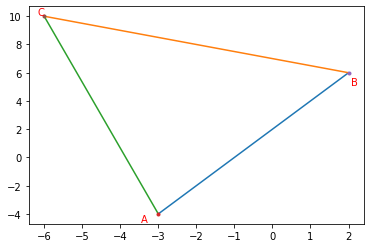
\includegraphics[width=0.5\textwidth]{Figure_1}
\caption{Right Angled Triangle\label{fig:triangle}}

\end{figure}
Say there exists two points $\textbf{P}(x_1, y_1)$ and $\textbf{Q}(x_2, y_2)$. The distance between the points is:
% Equation of y axis is 
\begin{align}
    \textbf{Z = P - Q}
\end{align}
Distance between \textbf{P} and \textbf{Q} is given by 
% For   $\Vec{
% 1 & -2 \\
% }x = 4$ (at y axis meet)
\begin{align}
||\textbf{Z}|| = \norm{\textbf{P-Q}}
\end{align}
% \begin{align}
% d = 
% \end{align}
Let $\textbf{P} = (-3, -4)$, $\textbf{Q} = (2, 6)$ and $\textbf{R} = (-6, 10)$.
\begin{enumerate}
    \item Distance between \textbf{P} and \textbf{Q} is 
\begin{align}
\norm{\textbf{P-Q}} = \sqrt{(-3-2)^2+(-4-6)^2}
=\sqrt{125}
\end{align}
\item Distance between \textbf{Q} and \textbf{R} is 
\begin{align}
\norm{\textbf{Q-R}} = \sqrt{(2-(-6))^2+(6-10)^2}
=\sqrt{80}
\end{align}
\item Distance between \textbf{P} and \textbf{R} is 
\begin{align}
\norm{\textbf{P-R}} = \sqrt{(-3-(-6))^2+(-4-10)^2}
=\sqrt{205}
\end{align}
\end{enumerate}
Here, the largest distance is $\sqrt{205}$. To be vertices of a right angled triangle, we should have 
\begin{align}
  \norm{\textbf{P-Q}}^2 + \norm{\textbf{Q-R}}^2 = \norm{\textbf{R-P}}^2
\end{align}
\begin{align}
  (\sqrt{205})^2 = (\sqrt{125})^2 + (\sqrt{80})^2
\end{align}
\begin{align}
  205 = 205
\end{align}
So, the condition is satisfied. 
So, using Baudhayana's theorem, it is proved that 3 points given are vertices of a right angled triangle. 
Now, for orthogonality, 
\begin{align}
    (\vec{P-Q})^T(\vec{Q-R}) = 0
\end{align}
We have 
\begin{enumerate}
    
    \item \begin{align}
    \vec{P-Q} = (2-(-3), 6-(-4))
\\
\vec{P-Q} = \myvec{
5\\
10 
}
\end{align}
    \item \begin{align}
    \vec{Q-R} = (2-(-6), 6-10)
\\
\vec{Q-R} = \myvec{
8\\
-4 
}
\end{align}
\item \begin{align}
    \vec{P-R} = (-3-(-6), -4-10)
\\
\vec{P-R} = \myvec{
3\\
-14 
}
\end{align}
\end{enumerate}
% We have 
% % \overrightarrow{\text {PQ}}
% \begin{align}
% \textbf{P}
% \\
%          \textbf{X}=(2-(-3), 6-(-4))
%  \\\textbf{X}= \myvec{
% 5\\
% 10 
% }
% \end{align}
% \overrightarrow{\text {QR}}
% Assuming Y is the vector, connecting Q and R. 
% \begin{align}
% \textbf{Y} = $$Q-R$$
% \\
%          \textbf{Y}=(2-(-6), 6-10)
%  \\\textbf{Y}= \myvec{
% 8\\
% -4 
% }
% \end{align}
% Assuming Z is the vector connecting P and R. 
% \begin{align}
% \textbf{Z} = $$P-R$$
% \\
%          \textbf{Z}=(-3-(-6), -4-10)
%  \\\textbf{Z}= \myvec{
% 3\\
% -14 
% }
% \end{align}
For orthogonality, product of transpose of one point and other must be 0. 
Here, checking for 
\begin{align}
    \myvec{
5\\
10 
}^T\myvec{ 8\\
-4
} =  \myvec{
5\\
10
}^T \myvec{
8 \\ -4
}=0
\end{align}
Hence, using orthogonality, it is proved that the points form a right angled triangle. 

\section{figure}

Figure \ref{fig:triangle} Right anlged triangle where A=P and B=Q and C=R


\end{document}